% !TEX encoding = UTF-8 Unicode
\documentclass[a4paper]{article}

\usepackage{color}
\usepackage{url}
\usepackage[utf8]{inputenc} % make weird characters work
\usepackage{graphicx}
%\usepackage[nottoc]{tocbibind}

\usepackage[serbian, english]{babel}

\usepackage[unicode]{hyperref}
\hypersetup{colorlinks,citecolor=green,filecolor=green,linkcolor=blue,urlcolor=blue}

% used for code
\usepackage{color}
\usepackage{listings}
\usepackage{setspace}

\definecolor{Background}{rgb}{0.97,0.97,0.97}

\renewcommand{\lstlistingname}{Code}
\lstdefinelanguage{Python3}{
	language=Python,
	firstnumber=1,
	stepnumber=1,
	numbers=left,
	numbersep=5pt, 
	tabsize=4,
	basicstyle=\small\ttfamily,	
	morekeywords={import,from,class,def,for,while,if,is,in,elif,else,not,and,or,print,break,
		continue,return,True,False,None,access,as,,del,except,exec,finally,global,import,lambda,pass,print,raise,try,assert},
	stringstyle=\color{mymauve},
	commentstyle=\color{mygreen},  
	keywordstyle=\color{blue},
	backgroundcolor=\color{Background},	
	captionpos=b,  
	frame=single,	  
 	breakatwhitespace=false,
 	breaklines=true,
 	escapeinside={\%*}{*)},
 	extendedchars=true,
 	keepspaces=true,
	numberstyle=\tiny\color{mygray},
  	rulecolor=\color{black},
  	showspaces=false,
  	showstringspaces=false,
  	showtabs=false,
}

% this will be used when we want to show results
\lstdefinelanguage{Print}{
	numbers=none,
	tabsize=4,
	basicstyle=\small\ttfamily,
	frame=none	
}

\definecolor{mygreen}{rgb}{0,0.6,0}
\definecolor{mygray}{rgb}{0.5,0.5,0.5}
\definecolor{mymauve}{rgb}{0.58,0,0.82}

\lstset{ 
                  % show the filename of files included with \lstinputlisting; also try caption instead of title
}

\begin{document}

\title{Mining NBA}
\author{David Gavrilović}
% \date{9.~april 2015.}
\maketitle
\thispagestyle{empty}

\newpage

\tableofcontents
\thispagestyle{empty}

\newpage

\section{Stats 101}
\label{Stats_101}

\subsection{Traditional stats}
\label{Traditional_stats}


\begin{itemize}
	\item \textbf{Pos} - Position. Traditionaly, position can be one of the following: \textit{\textbf{PG}} - point guard, \textit{\textbf{SG}} - shooting guard, \textit{\textbf{SF}} - small forward, \textit{\textbf{PF}} - power forward and \textit{\textbf{C}} - center. Nowdays, one player usually plays multiple positions and usually is one of the: \textit{\textbf{Point}} - primarly PG, \textit{\textbf{Combo guard}} - plays PG and SG, \textit{\textbf{Wing}} - SF and SG, \textit{\textbf{Forward}} - PF and SF, \textit{\textbf{Big}} - usually C but can also be PF.
	\item \textbf{G} - Games. Number of games player played in during a season.
	\item \textbf{GS} - Games started. Number of games player started. Cannot be greater than G.
	\item \textbf{MP} - Minutes played (Per game or total in a season).
	\item \textbf{FG} - Field goals.
	\item \textbf{FGA} - Field goals attempts.
	\item \textbf{FG\%} - Field goal percentage. Calculated as FG / FGA.
	\item \textbf{3P} - 3-point field goals.
	\item \textbf{3PA} - 3-point field goal attempts.
	\item \textbf{3P\%} - 3-point percentage. Calculated as 3P / 3PA.
	\item \textbf{2P} - 2-point field goals. 
	\item \textbf{2PA} - 2-point field goal attempts.
	\item \textbf{2P\%} - 2-point percentage. Calculated as 2P / 2PA.
	\item \textbf{FT} - Free throws.
	\item \textbf{FTA} - Free throw attempts.
	\item \textbf{FT\%} - Free throws percentage. Calculated as FT / FTA.
	\item \textbf{eFG\%} - Field goal percentage that takes into account that a 3-point field goal is, by one point, worth more than a 2-point field goal. Calculated as (FG + 0.5 * 3P) / FGA.
	\item \textbf{ORB} - Offensive rebounds.
	\item \textbf{TRB} - Defensive rebounds.
	\item \textbf{AST} - Assists.
	\item \textbf{STL} - Steals.
	\item \textbf{BLK} - Blocks.
	\item \textbf{TOV} - Turnovers.
	\item \textbf{PF} - Personal fouls.
	\item \textbf{PTS or PPG} - Points or Points per game.	
\end{itemize}	
	
\subsection{Advanced stats}
\label{Advanced_stats}

\begin{itemize}
	\item \textbf{ORtg} - Offensive rating. An estimate of points produced/scored by a player/team per 100 possessions \cite{odrt}.
	\item \textbf{DRtg} - Defensive rating. An estimate of point allowed per 100 possessions \cite{odrt}.  
	\item \textbf{PER} - Player efficiency rating. A measure of a per minute production standardized such that the league average is 15 \cite{per}.
	\item \textbf{TS\%} - True shooting percentage. Points per scoring attempt converted to the 2-point field goal percentage needed to score that many points per attempt. Calculated as  PTS / (2 *  FGA + 0.44 * FTA). 
	\item \textbf{3PAr} - 3-Point attempt rate. Percentage of FGA from 3-point range.
	\item \textbf{FTr} - Free throw attempt rate. Number of FTA per FGA.
	\item \textbf{ORD\%} - Offensive rebound percentage. An estimate of the percentage of available offensive rebounds a player grabbed while he was on the floor.
	\item \textbf{DRB\%} - Defensive rebound percentage. An estimate of the percentage of available defensive rebounds a player grabbed while he was on the floor
	\item \textbf{TRB\%} - Total rebound percentage. An estimate of the percentage of available rebounds a player grabbed while he was on the floor. 
	\item \textbf{AST\%} - Assist percentage. An estimate of the percentage of teammate field goals a player assisted while he was on the floor.
	\item \textbf{STL\%} - Steal Percentage. An estimate of the percentage of opponent possessions that end with a steal by the player while he was on the floor. 
	\item \textbf{BLK\%} - Block percentage. An estimate of the percentage of opponent two-point field goal attempts blocked by the player while he was on the floor. 
	\item \textbf{TOV\%} - Turnover percentage. An estimate of turnovers per 100 plays. 
	\item \textbf{USG\%} - Usage percentage. An estimate of the percentage of team plays used by a player while he was on the floor.  
	\item \textbf{OWS} - Offensive win shares. An estimate of the number of wins contributed by a player due to his offense \cite{ws}. 
	\item \textbf{DWS} - Defensive win shares. An estimate of the number of wins contributed by a player due to his defense \cite{ws}. 
	\item \textbf{WS} - Win shares. An estimate number of wins contibuted by a player \cite{ws}.
	\item \textbf{WS/48} - Win shares per 48 minutes. League average is around 0.100.
	\item \textbf{OBPM} - Offensive Box plus/minus. A box score estimate of the offensive points per 100 possessions that a player contributed above a league-average player, translated to an average team \cite{bpm}.
	\item \textbf{DBPM} - Defensive Box plus/minus. A box score estimate of the defensive points per 100 possessions that a player contributed above a league-average player, translated to an average team \cite{bpm}.
	\item \textbf{BPM} - Box plus/minus. A box score estimate of the points per 100 possessions that a player contributed above a league-average player, translated to an average team \cite{bpm}.
	\item \textbf{VORP} - Value over replacement player. An estimate of the points per 100 team possessions that a player contributed above a replacement-level (-2.0) player, translated to an average team and prorated to an 82-game season \cite{bpm}.

\end{itemize}

\section{Calculating prime of an average player}
\label{prime}

In this section we will try to determine when does an average player hit their \textit{prime}. But first, what is prime? In order to answer that question we must first define something called \textit{peak}. Peak is the best season player had in his career. Knowing that, prime can be defined as player's seasons in which he is close, or somewhat close, to his peak. Knowing length of a player's prime is important, because prime is probably the most important thing when discussing player's career. \\

In this research only individual statistics will be used in process of estimating prime years of a player. Because the ultimate stat that can correctly measure when do players hit their prime does not exist (yet), multiple other stats will be used, both traditional and advanced. Those stats are, mostly, PTS, FG and FGA from traditional and PER, WS, BPM and VORP from advanced stats. Reasoning behind first three is, well, player in his prime should be best version of himself, so he will probably score and shoot more than in his non-prime seasons. Stats such as PER, BPM and VORP exist so we could determine impact on a game by player, or how good a player is. Prime season should have higher values for this stat than for other seasons. WS is used to determine players contribution to winning. It's expected from a player to contribute to winning more in his prime years, than in the rest of his career. \\  

Of course, different players can hit their prime at different age. Let's check prime years of some of the players inducted, or soon to be inducted, into the Naismith memorial basketball hall of fame. Selected players are chosen without any particular reason. Players used are Bird (figure \ref{plt:bird}), Shaq (figure \ref{plt:shaq}) and Duncan (figure \ref{plt:duncan}). As we can see from the shown box plots, mentioned players had the best seasons when they were around 26 to 30 years old. From that we can conclude that those seasons were their prime.  \\


\begin{figure}[h!]
\begin{center}
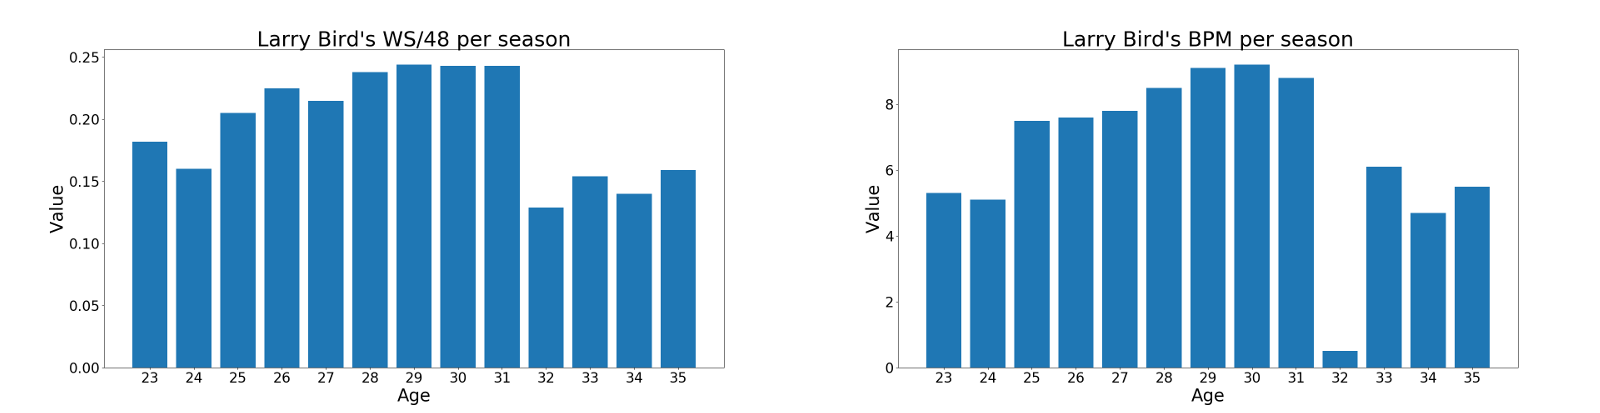
\includegraphics[scale=0.30]{bird.png}
\end{center}
\caption{Bird's WS/48 and BPM per season}
\label{plt:bird}
\end{figure}

\begin{figure}[h!]
\begin{center}
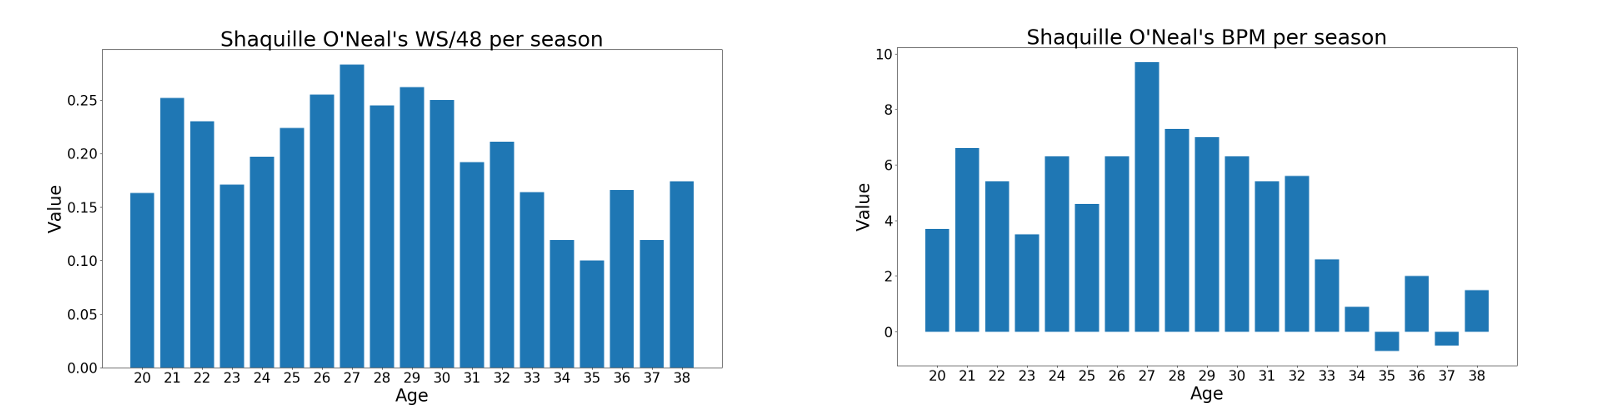
\includegraphics[scale=0.30]{shaq.png} % 2 x 800px and 413px
\end{center}
\caption{Shaq's WS/48 and BPM per season}
\label{plt:shaq}
\end{figure}

\begin{figure}[h!]
\begin{center}
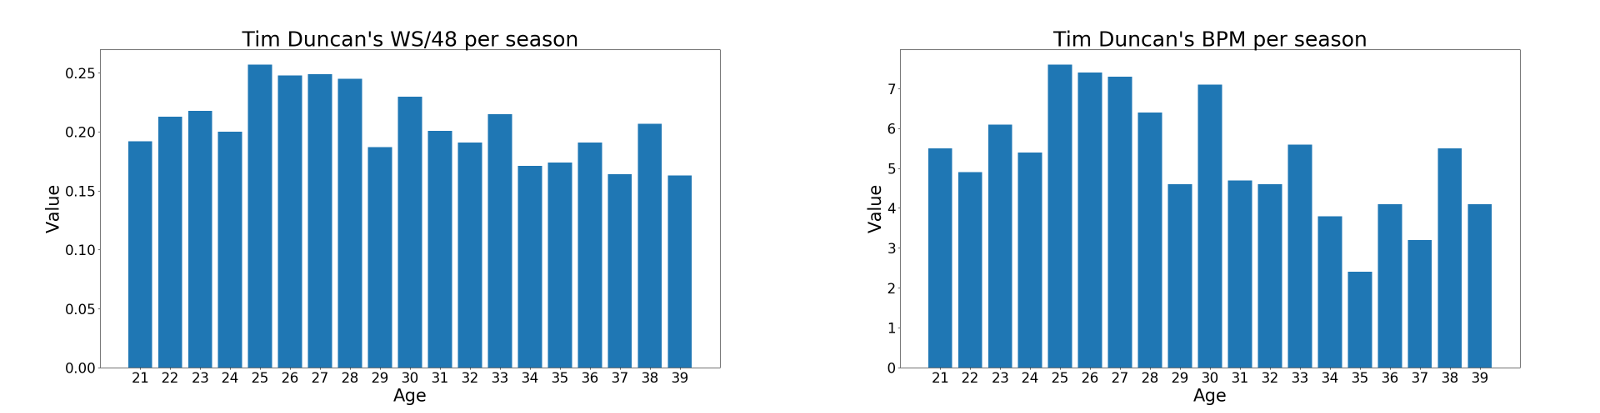
\includegraphics[scale=0.30]{duncan.png}
\end{center}
\caption{Duncan's WS/48 and BPM per season}
\label{plt:duncan}
\end{figure}


In the next step of determining prime of players, I checked at what age do players win awards, such as \textit{Regular season MVP}, \textit{Finals MVP}, \textit{DPOY} and \textit{Sixth man of the year} (\textit{SMOY}). Plots are shown in figure \ref{plt:awards}. Every plot but plot for Sixth man of the year is somewhat similar. The number of awards players won while in their late twenties and eary thirties is greater than number of awards in other years. Defensive player of the year award plot is different, where players aged from 23 to 31 won with roughly the same frequency, with an exception of players who were 28 (highest value) and 27 years old when they won. After that, there is a significant drop. These plots are showing us that the best players in the season are usually ones between 26 and 31 years old. But those players are stars and superstars. What about an average player?  \\

\begin{figure}[h!]
\begin{center}
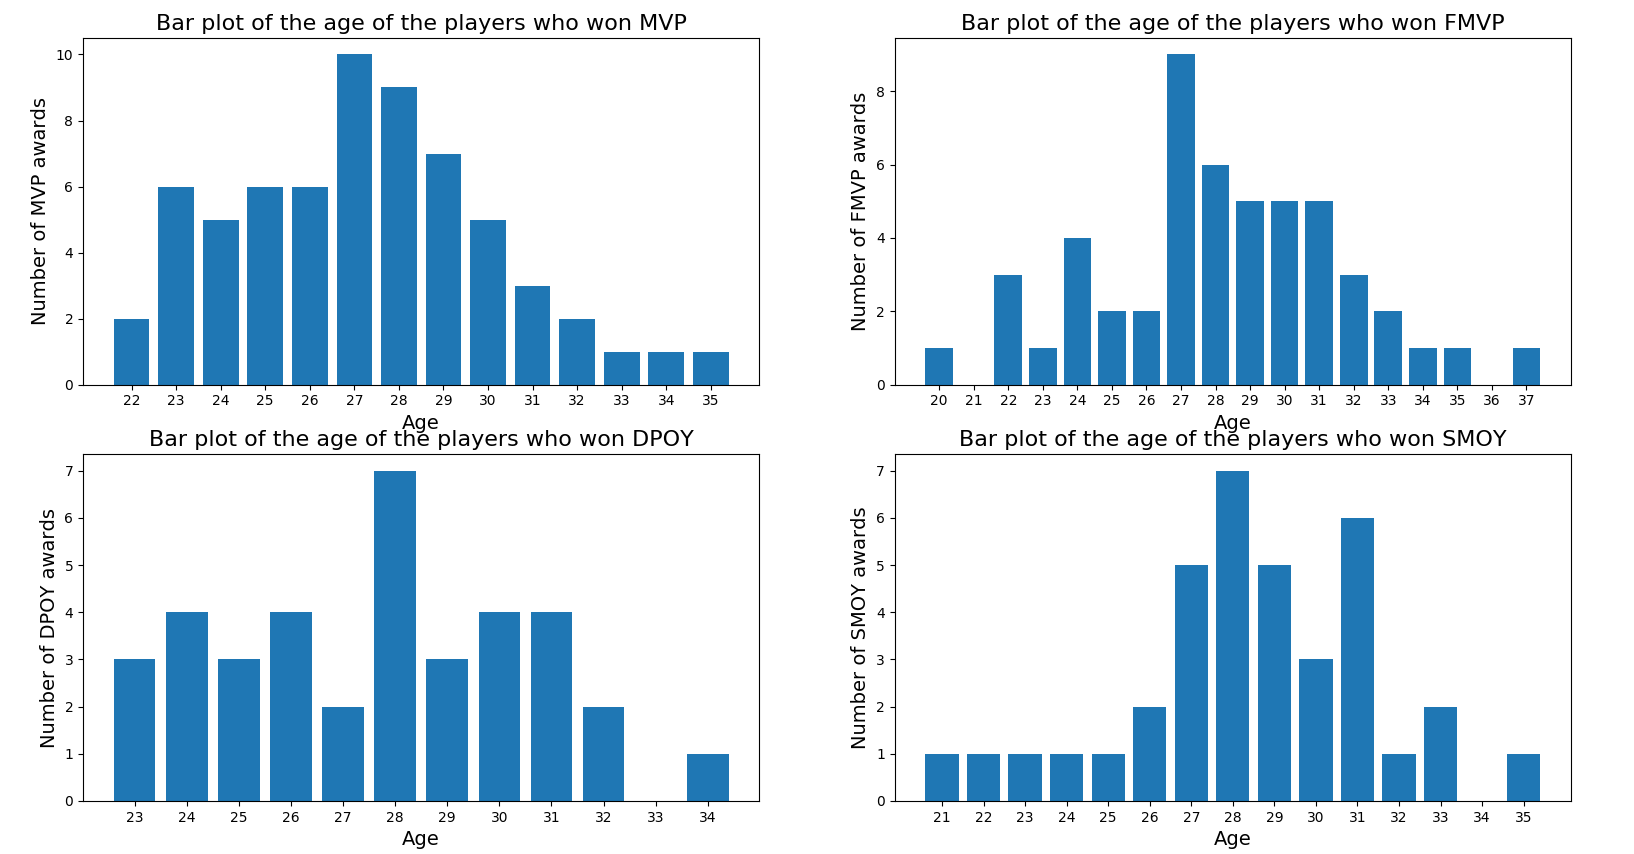
\includegraphics[scale=0.3]{awards_plots.png}
\end{center}
\caption{Age of award winners}
\label{plt:awards}
\end{figure}

After that, I checked age of players who played in the NBA. Results can be seen in figure \ref{plt:age_hist}. Note that there are two histograms. One represents every player who played in the NBA. The other is filtering out every player that has played in less than 25 games and less then 15 minutes per game. Those players are filtered out because I don't consider them regular contributors for the team they are playing for. The reason behind that is that they are probably not skilled enough, and possibly not in their prime, so they might not be important. Also, I just wanted to check on their histogram as well. Data used only takes into account players in the so-called \textit{Three-point era}. which began in 1979/80 season, the first season with 3-point line, and last till this day.

\begin{figure}[h!]
\begin{center}
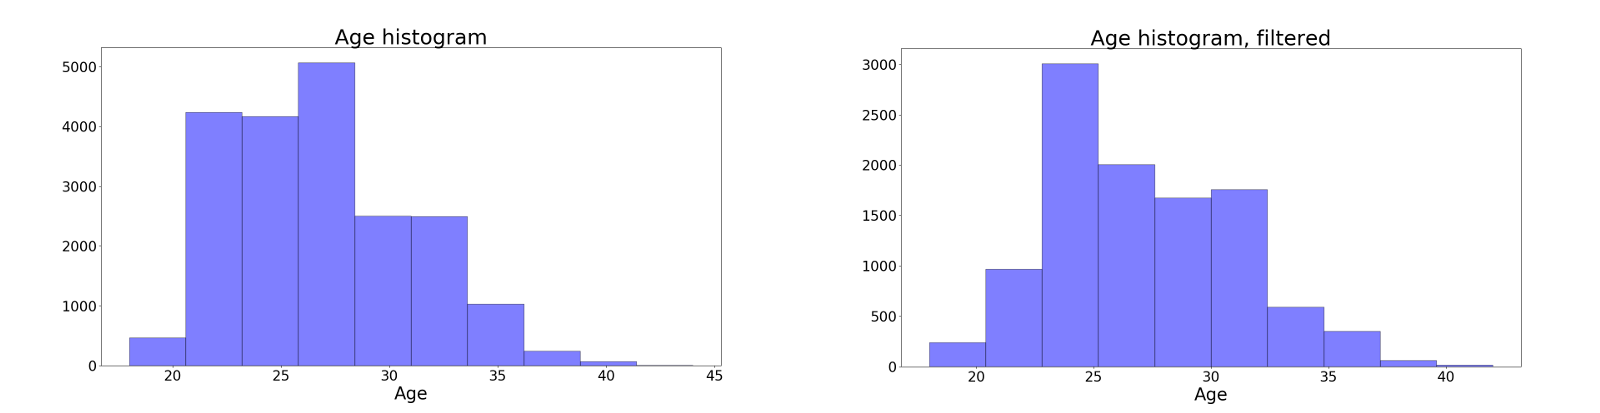
\includegraphics[scale=0.3]{age_histograms.png}
\end{center}
\caption{Age histograms}
\label{plt:age_hist}
\end{figure}


In the left histogram, unfiltered one, most of the players are in between 21 and 28 years old. That makes sense because players are usually drafted when they are younger than 25, and after rookie contracts expire and they are not good enough, they are out of the league. Histogram on the right has way lower number of players youger than around 23 years old. The reason behind that is that rookies aren't usually contributors right away because they need some time to develop.   The difference in number of players that are above 28 years old in unfiltered and filtered data is not that large. That is the case because players obove that age are usually good players, and they might be good because they are in their prime. That trend continues on both histograms until the significant drop somewhere after players reach 32 or 33. That might happen because they are simply not serviceable anymore, and because of that cannot find teams to sign with. 
To conclude this paragraph, number of players is rising ar first, until the age of 28. After that, there are two significant drops. \\

Now, I can try to estimate prime of an average player with statistics. First, I checked traditional stats. Box plots for four stats are shown, PTS, FG, FGA and FT. Simply, it is expected from a player in his prime to shoot and score more than in his non-prime seasons. Note that values represented on a y-axis are averages per season, not per game! In figure \ref{plt:totals_age} every player from the three-point era is taken into account while players represented in the figure \ref{plt:totals_age_filtered} are the ones I consider contributors (minutes per game $>$ 15 and games played $>$ 35). 

\begin{figure}[h!]
\begin{center}
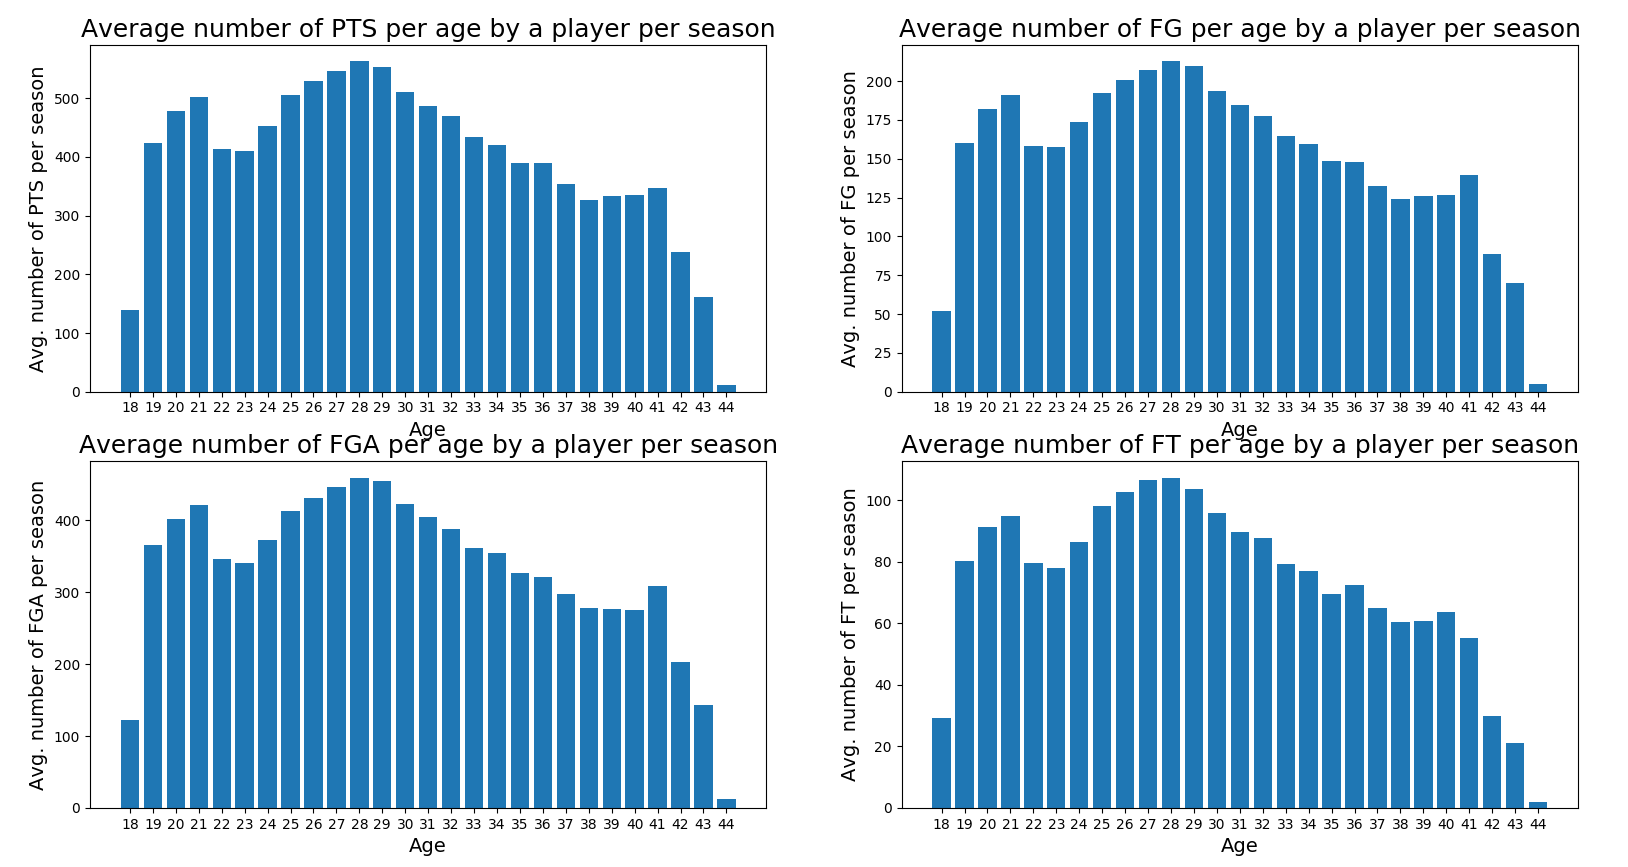
\includegraphics[scale=0.3]{traditional_stats_per_age.png}
\end{center}
\caption{Season totals averages per age unfiltered}
\label{plt:totals_age}
\end{figure}

\begin{figure}[h!]
\begin{center}
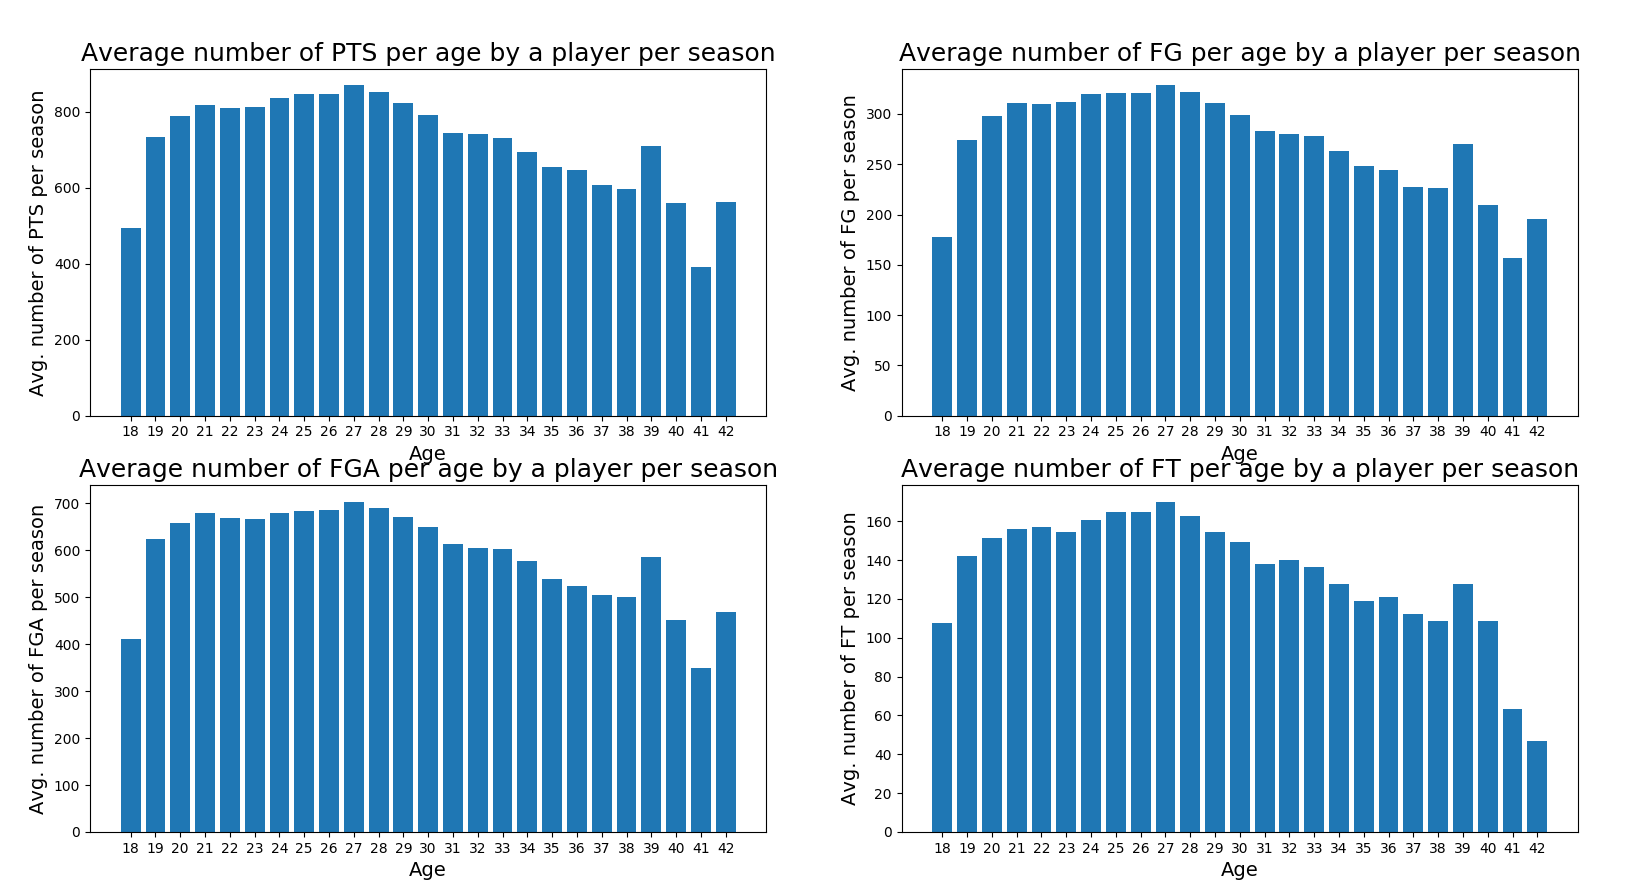
\includegraphics[scale=0.3]{traditional_stats_per_age_filtered.png}
\end{center}
\caption{Season totals averages per age filtered}
\label{plt:totals_age_filtered}
\end{figure}

Both plots are somewhat similar. Values for players age from 26 to 30 or maybe 31 are higher than for the any other age, with a significant drop after that. Both plots show peaks at a similar age, 28 for unfiltered data and 27 for filtered. So it's good thing to consider that prime of an average player is acually in late twenties/early thrties. The main difference can be seen in values for players that are younger than 25. Unfiltered data has a easily noticable difference between values for players 21 and players 22 years old. Reason behind that is probably draft. Promising players are drafted earlier, often before they are 20, while a lot of players with lower upside decide to devlop in college and try to enter the league later. Those players are the reason why the values are lower for certain age. From plots with filtered data we can observe that those players are not contributing right away, so lower values are, while still there, not so emphasized. \\

Advanced stats are better than traditional and hold more information about how good a certain player is. So, I did similar thing as in the paragraphs before, but now with the advanced stats. Stats chosen are PER, WS, BPM and VORP. Box plots for unfiltered players are shown in figure \ref{plt:advanced_age}, while box plots after filtering are in figure \ref{plt:advanced_age_filtered}.


\begin{figure}[h!]
\begin{center}
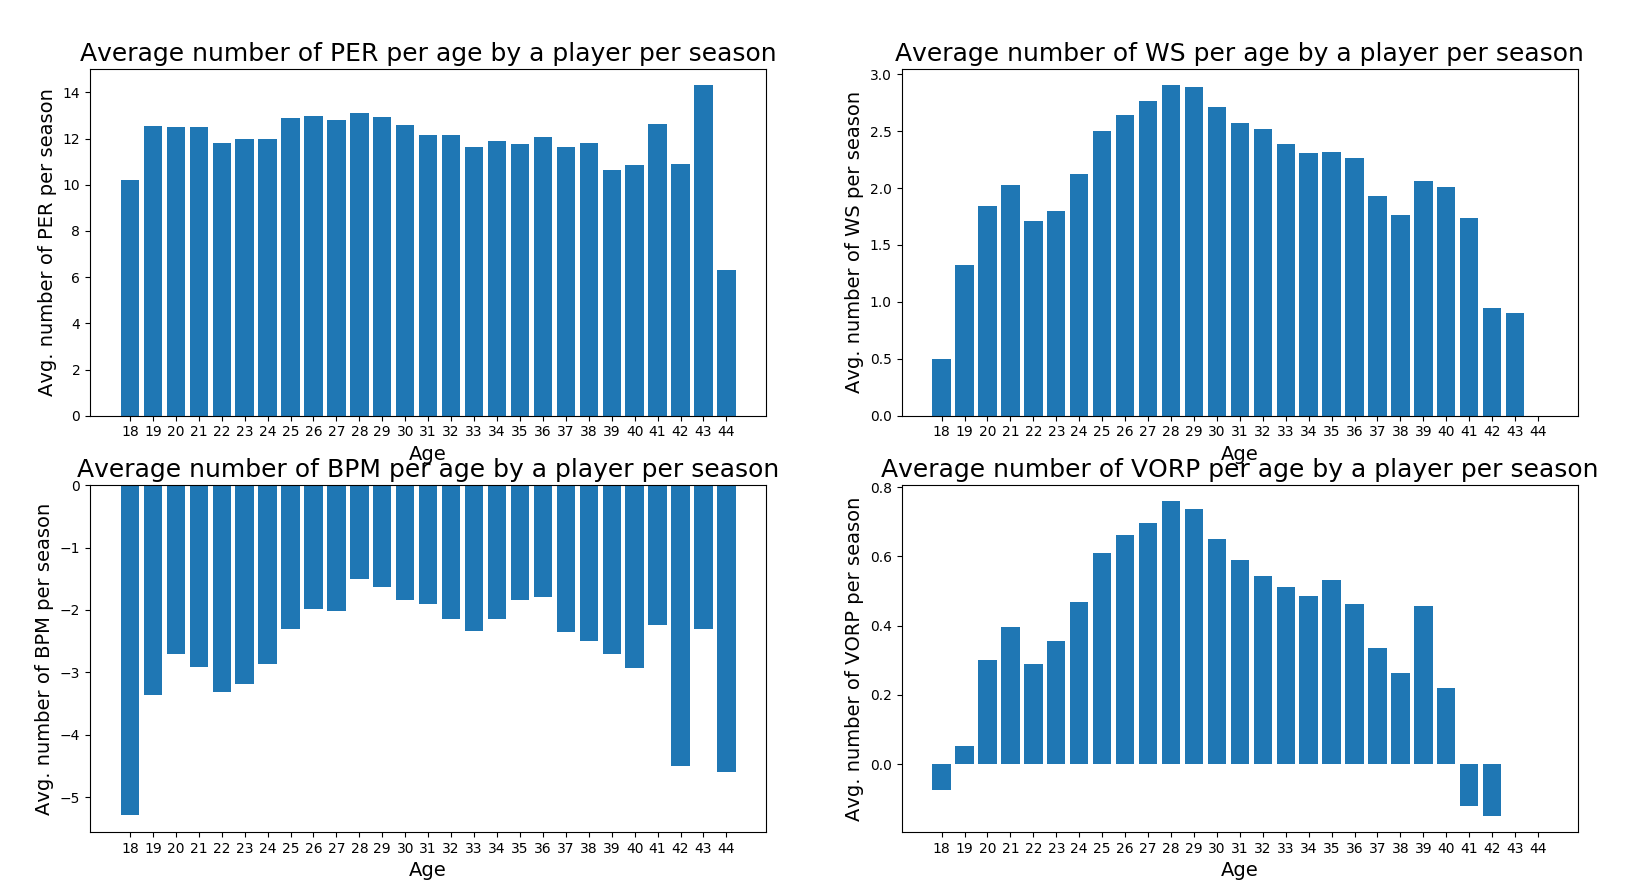
\includegraphics[scale=0.3]{advanced_stats_per_age.png}
\end{center}
\caption{Advanced stats averages per age unfiltered}
\label{plt:advanced_age}
\end{figure}

\begin{figure}[h!]
\begin{center}
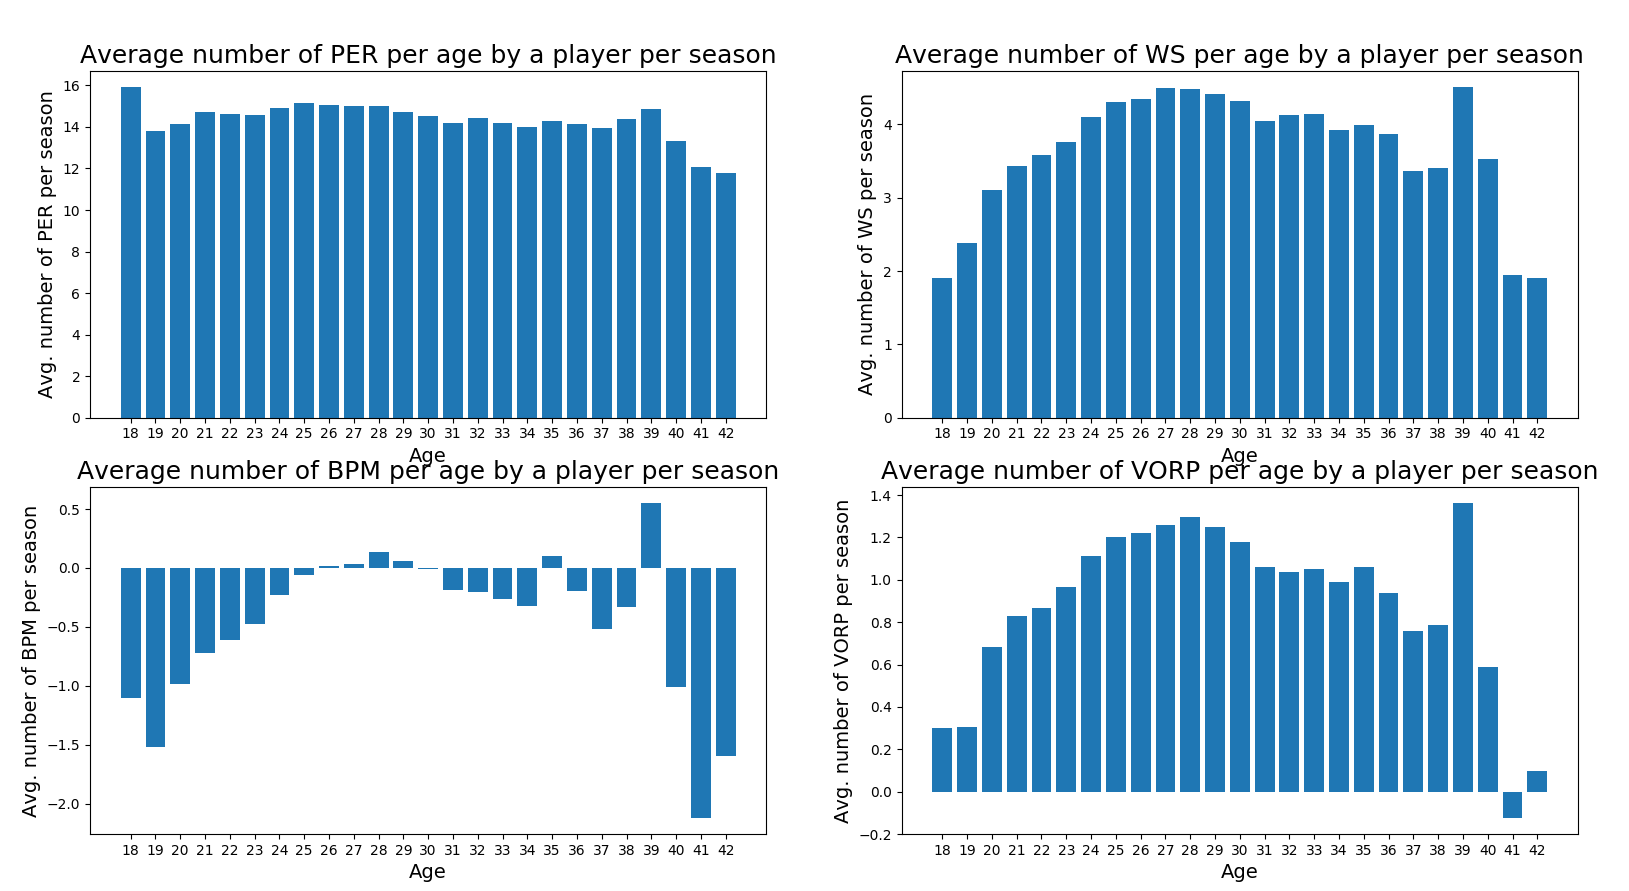
\includegraphics[scale=0.3]{advanced_stats_per_age_filtered.png}
\end{center}
\caption{Advanced stats averages per age filtered}
\label{plt:advanced_age_filtered}
\end{figure}

These plots are way more interesting. First, PER box plot, for both fitered and unfiltered data, is somewhat similar to the ones with traditional stats, with the same results. Plots for WS and VORP are \textbf{normal distribution-like}, with spike from 26 to 31 in y-axis values and lower values from the sides. That radius with higher values contains prime years af an average player. Plot for BPM is, interestinglly, negative for unfiltered data, and with some possitive values for filtered data. Highest values for BPM are from players from 25 to 36 years old. Some of the plots that are showing advanced data have high value for players 39 years old, wich is interesting. Those players were usually very good in their prime, and because of that they were usually good when they were older, just not that good anymore, and in usually lower minutes per game. It helps that there are not many players who played untill the age of 39. \\

Taking all mentioned things into a consideration, age when players are usually winning awards and age when the players are statistically better than in any other age, conclusion is that an average player enters into prime at around \textbf{25} year old, and exits when he is around \textbf{31}, with kinda significant drop after that. Peak season happens when player is from \textbf{27 to 29} years of age, somewhere in the middle of their prime.

\pagebreak

\addcontentsline{toc}{section}{References}
\appendix
\bibliography{ref}
\bibliographystyle{unsrt}
\appendix

\end{document}
